\phantomsection
\chapter{Face detection with Viola-Jones}
\label{chap:implementation_violajones}

\noindent The face detection part for this facial expression recognition system is based on Viola-Jones face detection algorithm. This chapter describes how this Viola-Jones algorithm is used and implemented.

\phantomsection
\section{Viola-Jones}

\vspace{\baselineskip}
\noindent To perform Viola-Jones face detection, video sequences of face are obtained with a webcam or the Kinect. The algorithm is then able to detect face and regions of interest in the frames, which are nose, left eye, right eye and mouth. 
\newline

\noindent Classifiers are trained prior to be used. They are then loaded with a model; one for the face and one for each ROI. Then, based on these classifiers, face and ROI are detected in the frames. Figure~\ref{violajones_implementation_example} shows an example of face and ROI detection. In this case of ROI detection, separate classifiers have been used for each eye. 
\newline

\begin{figure}[!h]
\begin{center}
\noindent 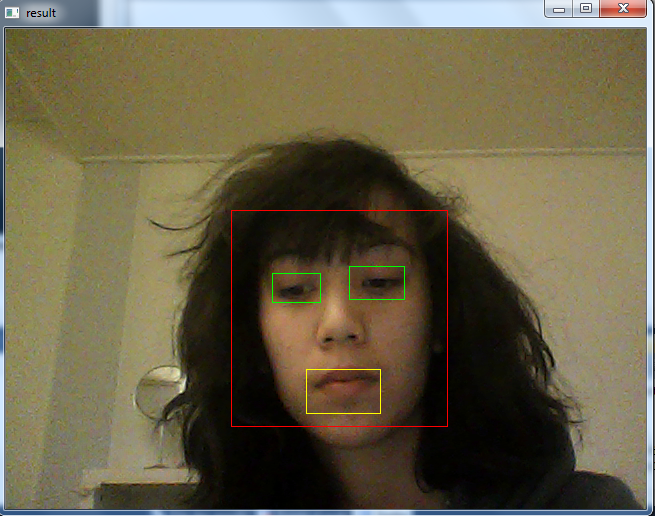
\includegraphics[scale=0.4]{figures/violajones_implementation_example} 
\newline
\caption{Example of face and ROI detection with Viola-Jones}
\label{violajones_implementation_example}
\end{center} 
\end{figure}

\noindent Detected faces are extracted with a size of $ 200\times200 $ pixels to discard as much background as possible, so they only contain the face and part of surrounding hair.